\documentclass[aspectratio=169,9pt,t]{beamer}

\usepackage[T1]{fontenc}
\usepackage{lmodern}
\usepackage{amsmath,amssymb,mathtools}
\usepackage{tikz}
\usetikzlibrary{arrows.meta,positioning,calc,fit}

% ---------- palette and Beamer setup ----------
\definecolor{Ink}{HTML}{172033}
\definecolor{Muted}{HTML}{5F6B7A}
\definecolor{Canvas}{HTML}{FAFAF7}
\definecolor{Graph}{HTML}{77736B}
\definecolor{LB}{HTML}{087D77}
\definecolor{LBSoft}{HTML}{E5F5F2}
\definecolor{Gold}{HTML}{B85F00}
\definecolor{GoldSoft}{HTML}{FFF3D6}

\usetheme{default}
\usefonttheme{professionalfonts}
\setbeamertemplate{navigation symbols}{}
\setbeamercolor{normal text}{fg=Ink,bg=Canvas}
\setbeamercolor{frametitle}{fg=Ink,bg=Canvas}
\setbeamercolor{statebar}{fg=Ink,bg=LBSoft}
\setbeamercolor{countbar}{fg=Ink,bg=white}
\setbeamercolor{explain}{fg=Ink,bg=white}
\setbeamercolor{takeaway}{fg=Ink,bg=GoldSoft}
\setbeamercolor{retained}{fg=Ink,bg=LBSoft}
\setbeamercolor{temporary}{fg=Ink,bg=GoldSoft}
\setbeamersize{text margin left=6mm,text margin right=6mm}
\setbeamertemplate{frametitle}{%
  \vspace{.6mm}\insertframetitle\par
  \vspace{.2mm}{\color{Graph}\rule{\textwidth}{0.4pt}}\vspace{-2.2mm}}
\setbeamertemplate{footline}{%
  \leavevmode\hbox{%
    \begin{beamercolorbox}[wd=.84\paperwidth,ht=2.5ex,dp=1.1ex,leftskip=6mm]{normal text}%
      \fontsize{5.8}{6.6}\selectfont\color{Muted}%
      Boundary-retained count excludes fixed $\boldsymbol\ell$, graph data, and temporary arithmetic; synchronized beats do not imply equal arithmetic, storage, or complexity
    \end{beamercolorbox}%
    \begin{beamercolorbox}[wd=.16\paperwidth,ht=2.5ex,dp=1.1ex,rightskip=6mm plus 1fil]{normal text}%
      \fontsize{6.2}{7.0}\selectfont\color{Muted}%
      Slide \insertframenumber\ of \inserttotalframenumber
    \end{beamercolorbox}}}

% ---------- fixed slide grammar ----------
\newcommand{\countstrip}[4]{%
  \begin{columns}[T,onlytextwidth]
    \column{.705\textwidth}
      \begin{beamercolorbox}[rounded=true,sep=.62ex]{statebar}
        \fontsize{6.4}{7.0}\selectfont\textcolor{Muted}{\bfseries SYNC BEAT #1 OF 7 \;·\; STATE NOW}\par
        \vspace{.15ex}\scriptsize #2
      \end{beamercolorbox}
    \column{.275\textwidth}
      \begin{beamercolorbox}[rounded=true,sep=.52ex]{countbar}
        \fontsize{6.4}{7.0}\selectfont\textcolor{LB}{\bfseries RETAINED NUMBERS}\par
        \fontsize{6.1}{6.8}\selectfont
        current $\mathbf{x}$: 3 \quad history: #3\par
        \textbf{retained now: #4}\quad / 63 configured cap
      \end{beamercolorbox}
  \end{columns}\vspace{.6mm}}

\newcommand{\phase}[1]{%
  \centering\colorbox{GoldSoft}{\strut\scriptsize\bfseries\textcolor{Gold}{#1}}\par\vspace{.6mm}}

\newcommand{\callout}[1]{%
  \begin{beamercolorbox}[rounded=true,sep=.65ex]{explain}
    \scriptsize #1
  \end{beamercolorbox}}

\newcommand{\takeaway}[1]{%
  \vspace{.3mm}\begin{beamercolorbox}[wd=\textwidth,rounded=true,sep=.6ex]{takeaway}
    \centering\scriptsize\bfseries #1
  \end{beamercolorbox}}

% ---------- diagram vocabulary ----------
\tikzset{
  bit/.style={circle,draw=LB,fill=white,line width=1.15pt,minimum size=8.5mm,inner sep=0pt,font=\scriptsize\bfseries},
  check/.style={rectangle,draw=LB,fill=LBSoft,line width=1.15pt,minimum width=8.5mm,minimum height=7.5mm,rounded corners=1.3pt,inner sep=0pt,font=\scriptsize\bfseries},
  edge/.style={draw=Graph!55,line width=1.1pt},
  activeedge/.style={draw=LB!32,line width=3.1pt},
  dependency/.style={draw=LB,line width=1.8pt,dashed},
  valuechip/.style={fill=white,draw=LB,rounded corners=1.6pt,inner xsep=1.8pt,inner ysep=1pt,font=\fontsize{6.5}{7}\selectfont,text=Ink},
  tempchip/.style={fill=GoldSoft,draw=Gold,dashed,rounded corners=1.6pt,inner xsep=1.8pt,inner ysep=1pt,font=\fontsize{6.5}{7}\selectfont,text=Gold},
  flowretain/.style={draw=LB,fill=LBSoft,line width=1.1pt,rounded corners=2.5pt,minimum height=12mm,text width=34mm,align=center,font=\scriptsize},
  flowtemp/.style={draw=Gold,fill=GoldSoft,dashed,line width=1.1pt,rounded corners=2.5pt,minimum height=12mm,text width=34mm,align=center,font=\scriptsize},
  flowarrow/.style={draw=LB,line width=1.35pt,-{Stealth[length=2.5mm]}},
  looparrow/.style={draw=Gold,line width=1.25pt,-{Stealth[length=2.5mm]}}
}

\newcommand{\lbgraph}[3]{%
  \node[check] (A) at (-1.7,1.65) {$A$};
  \node[check] (B) at ( 1.7,1.65) {$B$};
  \node[bit] (b1) at (-3.0,0) {bit 1};
  \node[bit] (b2) at ( 0.0,0) {bit 2};
  \node[bit] (b3) at ( 3.0,0) {bit 3};
  \draw[edge] (A)--(b1);
  \draw[edge] (A)--(b2);
  \draw[edge] (B)--(b2);
  \draw[edge] (B)--(b3);
  \node[below=3.5mm of b1,font=\tiny] {$x_1=#1$};
  \node[below=3.5mm of b2,font=\tiny] {$x_2=#2$};
  \node[below=3.5mm of b3,font=\tiny] {$x_3=#3$};
}

\newcommand{\graphstart}{\begin{tikzpicture}[x=.92cm,y=.92cm]}
\newcommand{\graphend}{\end{tikzpicture}}

\begin{document}

% Slide 1 — synchronized with BP slide 1
\begin{frame}{L-BFGS in one loop: evaluate, move, and remember}
  \countstrip{1}{\textbf{ITERATION BOUNDARY: }retain one scalar vector $\mathbf{x}^{(t)}$ and up to ten accepted $\bigl(\mathbf{s},\mathbf{y}\bigr)$ history pairs. All check terms are recalculated.}{0 scalars}{3}

  \phase{EVALUATE AT FROZEN $\mathbf{x}^{(t)}$ \quad $\longrightarrow$ \quad FORM A DIRECTION \quad $\longrightarrow$ \quad ACCEPT A PROJECTED STEP \quad $\longrightarrow$ \quad REPEAT}

  \begin{columns}[T,onlytextwidth]
    \column{.43\textwidth}
      \centering
      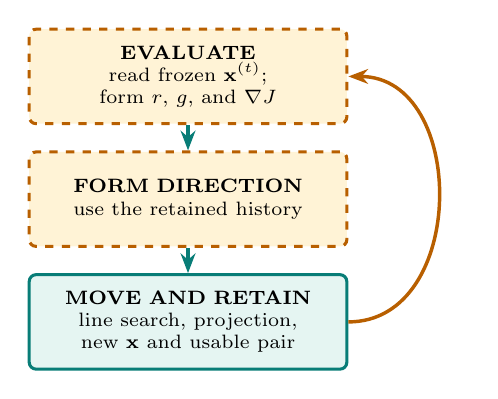
\begin{tikzpicture}[node distance=3.2mm]
        \node[flowtemp,text width=38mm] (eval)
          {\textbf{EVALUATE}\par read frozen $\mathbf{x}^{(t)}$; form $r$, $g$, and $\nabla J$};
        \node[flowtemp,text width=38mm,below=of eval] (direction)
          {\textbf{FORM DIRECTION}\par use the retained history};
        \node[flowretain,text width=38mm,below=of direction] (move)
          {\textbf{MOVE AND RETAIN}\par line search, projection, new $\mathbf{x}$ and usable pair};
        \draw[flowarrow] (eval)--(direction);
        \draw[flowarrow] (direction)--(move);
        \draw[looparrow] (move.east) to[out=0,in=0,looseness=1.25] (eval.east);
      \end{tikzpicture}
    \column{.55\textwidth}
      \callout{\centering\textbf{Objective function in this three-bit teaching variant}\par
        \[
          J(\mathbf{x})=-\frac12\sum_{i=1}^{3}\ell_i x_i
          +2\!\sum_{c\in\{A,B\}}\!\left(1-\prod_{j\in c}x_j\right)^2
        \]}
      \vspace{.7mm}
      \callout{\centering\textbf{One accepted update}\par
        \[
          \mathbf{d}^{(t)}=-\mathbf{H}_t\nabla J(\mathbf{x}^{(t)}),\qquad
          \mathbf{x}^{(t+1)}=\Pi_{[-1,1]^3}
          \bigl(\mathbf{x}^{(t)}+\alpha_t\mathbf{d}^{(t)}\bigr)
        \]}
  \end{columns}

  \takeaway{L-BFGS retains one current scalar per bit and accepted history pairs; its temporary check calculations are not Tanner-graph messages.}
\end{frame}

% Slide 2 — synchronized with BP slide 2
\begin{frame}{Initialize once: channel evidence and one scalar per bit}
  \countstrip{2}{\textbf{INITIAL VALUES: }fixed $\boldsymbol\ell=-\mathbf{L}$, current $\mathbf{x}^{(0)}=\tanh(\boldsymbol\ell/2)$, and an empty L-BFGS history.}{0 scalars}{3}

  \phase{PLACE FIXED $\boldsymbol\ell$ \quad $\longrightarrow$ \quad INITIALIZE $\mathbf{x}^{(0)}$ \quad $\longrightarrow$ \quad KEEP ONE SCALAR PER BIT}

  \begin{columns}[T,onlytextwidth]
    \column{.58\textwidth}
      \centering
      \graphstart
        \lbgraph{+0.800}{-0.200}{-0.333}
        \node[below=8.2mm of b1,font=\tiny,text=Muted] {$\ell_1=+2.197$};
        \node[below=8.2mm of b2,font=\tiny,text=Muted] {$\ell_2=-0.405$};
        \node[below=8.2mm of b3,font=\tiny,text=Muted] {$\ell_3=-0.693$};
      \graphend
    \column{.40\textwidth}
      \callout{\centering
        \[
          \boldsymbol\ell=-\mathbf{L}
          =(+2.197,-0.405,-0.693)
        \]
        \[
          \mathbf{x}^{(0)}=\tanh(\boldsymbol\ell/2)
          =(+0.800,-0.200,-0.333)
        \]}
      \vspace{1mm}
      \begin{beamercolorbox}[rounded=true,sep=.75ex]{retained}
        \scriptsize\textcolor{LB}{\bfseries BOUNDARY-RETAINED NUMBERS}\par\vspace{.4mm}
        \fontsize{7.2}{8.2}\selectfont
        $\mathbf{x}^{(0)}[3]$ \hfill 3 scalars\par
        history pairs \hfill $0/10$\par
        configured cap \hfill $3+2(3)(10)=63$
      \end{beamercolorbox}
  \end{columns}

  \takeaway{Here $\ell_i>0$ and $x_i>0$ favour bit 0; the BP deck uses the opposite-sign channel LLR $L_i=-\ell_i$.}
\end{frame}

% Slide 3 — synchronized with BP slide 3
\begin{frame}{Frozen-state read: both checks evaluate their residuals}
  \countstrip{3}{\textbf{LOCKED READ: }checks A and B both use the same frozen $\mathbf{x}^{(0)}$. The two residuals are temporary calculations.}{0 scalars}{3}

  \phase{LOCK $\mathbf{x}^{(0)}$ \quad $\longrightarrow$ \quad A READS $x_1,x_2$ \quad + \quad B READS $x_2,x_3$ \quad $\longrightarrow$ \quad FORM $r_A,r_B$}

  \begin{columns}[T,onlytextwidth]
    \column{.58\textwidth}
      \centering
      \graphstart
        \lbgraph{+0.800}{-0.200}{-0.333}
        \draw[activeedge] (A)--(b1); \draw[activeedge] (A)--(b2);
        \draw[activeedge] (B)--(b2); \draw[activeedge] (B)--(b3);
        \draw[dependency] (A)--(b1); \draw[dependency] (A)--(b2);
        \draw[dependency] (B)--(b2); \draw[dependency] (B)--(b3);
        \node[draw=Gold,circle,line width=1.5pt,minimum size=11mm,fit=(b2),inner sep=0pt] {};
        \node[tempchip,above=5mm of A] {$r_A=1.160$};
        \node[tempchip,above=5mm of B] {$r_B=0.933333$};
      \graphend
    \column{.40\textwidth}
      \callout{\centering
        \[
          r_c=1-\prod_{j\in c}x_j
        \]}
      \vspace{.8mm}
      \callout{\centering
        $\begin{aligned}
          r_A&=1-(0.800)(-0.200)=1.160,\\
          r_B&=1-(-0.200)(-0.333333)=0.933333.
        \end{aligned}$}
      \vspace{.8mm}
      \begin{beamercolorbox}[rounded=true,sep=.65ex]{takeaway}
        \centering\scriptsize\bfseries
        A then B is presentation order. Neither check updates $\mathbf{x}^{(0)}$.
      \end{beamercolorbox}
  \end{columns}

  \takeaway{The dashed lines show mathematical dependence on the frozen coordinates; no value travels along a Tanner-graph edge.}
\end{frame}

% Slide 4 — synchronized with BP slide 4
\begin{frame}{Check contributions: four temporary terms for the partial derivatives}
  \countstrip{4}{\textbf{ONE FROZEN SNAPSHOT: }the four $g_{c,i}$ values all use $\mathbf{x}^{(0)}$. They are combined later by bit coordinate and are not retained across the boundary.}{0 scalars}{3}

  \phase{READ FROZEN $\mathbf{x}^{(0)}$ AND $r_c$ \quad $\longrightarrow$ \quad FORM FOUR $g_{c,i}$ TERMS \quad $\longrightarrow$ \quad KEEP $\mathbf{x}^{(0)}$ FIXED}

  \begin{columns}[T,onlytextwidth]
    \column{.58\textwidth}
      \centering
      \graphstart
        \lbgraph{+0.800}{-0.200}{-0.333}
        \draw[activeedge] (A)--(b1); \draw[activeedge] (A)--(b2);
        \draw[activeedge] (B)--(b2); \draw[activeedge] (B)--(b3);
        \node[tempchip] at ($(A)!.53!(b1)+(-.15,.05)$) {$g_{A,1}$};
        \node[tempchip] at ($(A)!.53!(b2)+(-.12,.05)$) {$g_{A,2}$};
        \node[tempchip] at ($(B)!.53!(b2)+(.12,.05)$) {$g_{B,2}$};
        \node[tempchip] at ($(B)!.53!(b3)+(.15,.05)$) {$g_{B,3}$};
      \graphend
    \column{.40\textwidth}
      \callout{\centering
        \[
          g_{c,i}=-4r_c\!\!\prod_{\substack{j\in c\\j\ne i}}\!x_j
        \]}
      \vspace{.7mm}
      \begin{columns}[T,onlytextwidth]
        \column{.49\textwidth}
          \callout{\centering\textbf{check A}\par
            $\begin{aligned}
              g_{A,1}&=+0.928,\\
              g_{A,2}&=-3.712
            \end{aligned}$}
        \column{.49\textwidth}
          \callout{\centering\textbf{check B}\par
            $\begin{aligned}
              g_{B,2}&=+1.244,\\
              g_{B,3}&=+0.747
            \end{aligned}$}
      \end{columns}
      \vspace{.7mm}
      \callout{\centering The terms are indexed by check and coordinate only while the partial derivatives are being calculated.}
  \end{columns}

  \takeaway{These four values contribute to $\nabla J$; they are temporary partial-derivative terms, not directed messages.}
\end{frame}

% Slide 5 — synchronized with BP slide 5
\begin{frame}{Aggregate by coordinate, choose a direction, then move once}
  \countstrip{5}{\textbf{START: }$\mathbf{x}^{(0)}$ stays frozen while $\nabla J$, $\mathbf{d}^{(0)}$, and the trial steps are formed. \textbf{END: }the accepted point $\mathbf{x}^{(1)}$ becomes current.}{0 scalars}{3}

  \phase{ASSEMBLE $\nabla J$ \quad $\longrightarrow$ \quad $\mathbf{d}^{(0)}=-\nabla J$ \quad $\longrightarrow$ \quad LINE SEARCH \quad $\longrightarrow$ \quad PROJECT AND MOVE}

  \begin{columns}[T,onlytextwidth]
    \column{.53\textwidth}
      \callout{\centering\textbf{Combine all terms by bit coordinate}\par
        \[
          \nabla J(\mathbf{x}^{(0)})=
          \begin{bmatrix}
            g_{A,1}-\tfrac12\ell_1\\
            g_{A,2}+g_{B,2}-\tfrac12\ell_2\\
            g_{B,3}-\tfrac12\ell_3
          \end{bmatrix}
          =\begin{bmatrix}-0.170612\\-2.264823\\+1.093240\end{bmatrix}
        \]}
      \vspace{.6mm}
      \callout{\centering
        $\mathbf{H}_0=\mathbf{I}$ because the history is empty, so
        \[
          \mathbf{d}^{(0)}=-\nabla J
          =(+0.170612,+2.264823,-1.093240).
        \]}
      \vspace{.6mm}
      \begin{beamercolorbox}[rounded=true,sep=.65ex]{temporary}
        \centering\scriptsize
        $\alpha=1$: $J=6.791560$ reject \quad
        $\alpha=0.5$: $J=5.600661$ reject\par
        $\alpha=0.25$: $J=2.881689<3.398461$ \textbf{accept}
      \end{beamercolorbox}
    \column{.45\textwidth}
      \centering
      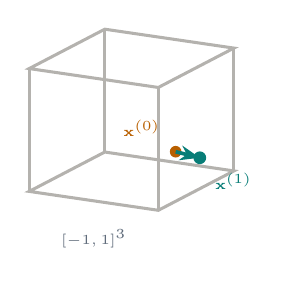
\begin{tikzpicture}[x={(.82cm,-.12cm)},y={(.48cm,.25cm)},z={(0cm,.78cm)}]
        \coordinate (mmm) at (-1,-1,-1); \coordinate (pmm) at (1,-1,-1);
        \coordinate (mpm) at (-1,1,-1);  \coordinate (ppm) at (1,1,-1);
        \coordinate (mmp) at (-1,-1,1);  \coordinate (pmp) at (1,-1,1);
        \coordinate (mpp) at (-1,1,1);   \coordinate (ppp) at (1,1,1);
        \draw[edge] (mmm)--(pmm)--(ppm)--(mpm)--cycle;
        \draw[edge] (mmp)--(pmp)--(ppp)--(mpp)--cycle;
        \draw[edge] (mmm)--(mmp); \draw[edge] (pmm)--(pmp);
        \draw[edge] (mpm)--(mpp); \draw[edge] (ppm)--(ppp);
        \coordinate (xzero) at (.8,-.2,-.333333);
        \coordinate (xone) at (.842653,.366206,-.606643);
        \fill[Gold] (xzero) circle (2.1pt) node[above left=1mm,font=\tiny] {$\mathbf{x}^{(0)}$};
        \draw[flowarrow] (xzero)--(xone);
        \fill[LB] (xone) circle (2.3pt) node[below right=1mm,font=\tiny] {$\mathbf{x}^{(1)}$};
        \node[font=\tiny,text=Muted] at (0,-1,-1.62) {$[-1,1]^3$};
      \end{tikzpicture}
      \vspace{.7mm}
      \callout{\centering
        \[
          \begin{aligned}
            \mathbf{x}^{(1)}
              &=\Pi\!\left(\mathbf{x}^{(0)}+0.25\mathbf{d}^{(0)}\right)\\
              &=(+0.842653,+0.366206,-0.606643)
          \end{aligned}
        \]
        The accepted $\alpha=0.25$ trial is inside the box, so the projection changes nothing.}
  \end{columns}
\end{frame}

% Slide 6 — synchronized with BP slide 6
\begin{frame}{Next evaluation: both checks still read one bit-2 scalar}
  \countstrip{6}{\textbf{FORM THE FIRST HISTORY PAIR: }start with $\mathbf{x}^{(1)}$. Both checks read the same $x_2^{(1)}$ to assemble $\nabla J(\mathbf{x}^{(1)})$; only then can the usable pair be retained.}{0 $\to$ 6 scalars}{3 $\to$ 9 by beat end}

  \phase{KEEP $\mathbf{x}^{(1)}$ (3) \; $\longrightarrow$ \; BOTH CHECKS READ $x_2^{(1)}$ AND FORM $\nabla J(\mathbf{x}^{(1)})$ \; $\longrightarrow$ \; FORM AND RETAIN THE PAIR (9) \; $\longrightarrow$ \; FORM $\mathbf{d}^{(1)}$}

  \begin{columns}[T,onlytextwidth]
    \column{.58\textwidth}
      \centering
      \graphstart
        \lbgraph{+0.843}{+0.366}{-0.607}
        \draw[activeedge] (A)--(b2); \draw[activeedge] (B)--(b2);
        \draw[dependency] (A)--(b2); \draw[dependency] (B)--(b2);
        \node[draw=Gold,circle,line width=1.6pt,minimum size=11mm,fit=(b2),inner sep=0pt] {};
        \node[valuechip,above=5mm of A] {$A$ reads $x_2^{(1)}=+0.366$};
        \node[valuechip,above=5mm of B] {$B$ reads $x_2^{(1)}=+0.366$};
        \node[font=\large\bfseries,text=LB] at (0,1.65) {$=$};
      \graphend
    \column{.40\textwidth}
      \callout{\centering
        \textbf{1. Finish the new evaluation}\par
        $\nabla J(\mathbf{x}^{(1)})=(-2.111,+0.838,-1.444)$
        \par\vspace{1mm}
        \textbf{2. Only now form the history pair}\par
        $\mathbf{s}^{(0)}=(+0.043,+0.566,-0.273)$\par
        $\mathbf{y}^{(0)}=(-1.941,+3.103,-2.537)$\par
        \fontsize{6.4}{7.1}\selectfont
        $\mathbf{y}^{(0)}=\nabla J(\mathbf{x}^{(1)})-\nabla J(\mathbf{x}^{(0)})$
        \par\vspace{1mm}
        \scriptsize\textbf{3. Test, retain, then use the pair}\par
        $(\mathbf{s}^{(0)})^{\!T}\mathbf{y}^{(0)}=2.367356>10^{-12}$\par
        $\mathbf{d}^{(1)}=(+0.170,-0.055,+0.110)$}
  \end{columns}

  \takeaway{Unlike BP's two recipient-specific $Q$ values from bit 2, L-BFGS retains one $x_2$ value and both checks read that value.}
\end{frame}

% Slide 7 — synchronized with BP slide 7
\begin{frame}{What crosses an L-BFGS iteration boundary}
  \countstrip{7}{\textbf{AFTER THE FIRST PAIR: }$\mathbf{x}^{(1)}$, $\mathbf{s}^{(0)}$, and $\mathbf{y}^{(0)}$ cross the boundary. Residuals, check terms, the gradient, and the direction are recalculated.}{6 scalars}{9}

  \phase{KEEP $\mathbf{x}$ AND ACCEPTED HISTORY \quad $\longrightarrow$ \quad RECALCULATE TEMPORARY TERMS \quad $\longrightarrow$ \quad ACCEPT THE NEXT UPDATE}

  \begin{columns}[T,onlytextwidth]
    \column{.45\textwidth}
      \centering
      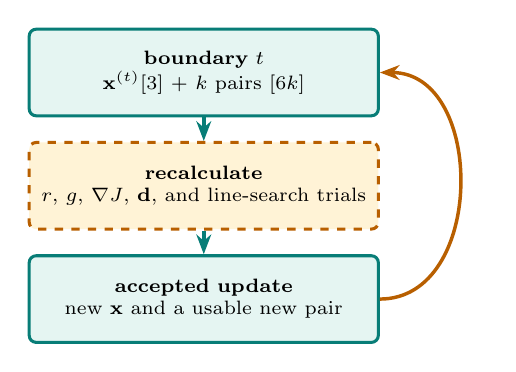
\begin{tikzpicture}[node distance=3mm]
        \node[flowretain,text width=42mm,minimum height=11mm] (boundary)
          {\textbf{boundary $t$}\\$\mathbf{x}^{(t)}[3]$ + $k$ pairs $[6k]$};
        \node[flowtemp,text width=42mm,minimum height=11mm,below=of boundary] (work)
          {\textbf{recalculate}\\$r$, $g$, $\nabla J$, $\mathbf{d}$, and line-search trials};
        \node[flowretain,text width=42mm,minimum height=11mm,below=of work] (next)
          {\textbf{accepted update}\\new $\mathbf{x}$ and a usable new pair};
        \draw[flowarrow] (boundary)--(work);
        \draw[flowarrow] (work)--(next);
        \draw[looparrow] (next.east) to[out=0,in=0,looseness=1.20] (boundary.east);
      \end{tikzpicture}
      \vspace{1mm}
      \begin{beamercolorbox}[rounded=true,sep=.8ex]{temporary}
        \centering\scriptsize
        Check A then check B is only presentation order: both evaluations use the same frozen iterate.
      \end{beamercolorbox}
    \column{.53\textwidth}
      \begin{beamercolorbox}[rounded=true,sep=.8ex]{retained}
        \scriptsize\textcolor{LB}{\bfseries RETAINED AFTER THE FIRST ACCEPTED PAIR}\par\vspace{.5mm}
        \fontsize{7.2}{8.3}\selectfont
        $\mathbf{x}^{(1)}[3]$ \hfill 3 coordinate values\par
        $\mathbf{s}^{(0)}[3]$ \hfill 3 history values\par
        $\mathbf{y}^{(0)}[3]$ \hfill 3 history values\par
        \textbf{retained now} \hfill \textbf{9 scalar values}
      \end{beamercolorbox}
      \vspace{1mm}
      \begin{beamercolorbox}[rounded=true,sep=.8ex]{temporary}
        \scriptsize\textcolor{Gold}{\bfseries GENERAL BOUNDARY COUNT}\par\vspace{.5mm}
        \fontsize{7.2}{8.3}\selectfont
        $3+6k$ retained scalars for $k$ history pairs\par
        $0\le k\le10$; configured cap $=3+6(10)=63$\par
        fixed $\boldsymbol\ell$, graph data, and temporary arithmetic excluded
      \end{beamercolorbox}
      \vspace{1mm}
      \callout{\centering The retained state is indexed by bit coordinate and update history, not by Tanner-graph edge. In this constructed teaching variant, the displayed $J$ is three times the anchored channel-rung objective and has no binary term; it is a mechanism tutorial, not performance evidence.}
  \end{columns}
\end{frame}

\end{document}
